\chapter{Related Work} \label{ch:related_work}
\section{SDN}



\section{OpenFlow}



\section{NFV}



\section{Related vCPE framework}
\subsection{Cloud4NFV}


\subsection{NetFate}


\subsection{Ericsson CPE}



\section{HSNL vCPE framework}
The following part of this paper moves on to describe in greater detail the HSNL vCPE framework. Our proposed vCPE functions, which is implementd by multiple flow table management mechanism, also can be deployed by this framework.


\subsection{Deploymeny Model}
Unlike a related study that explored the virtualization of network function in PE devices \cite{vcpe-enhance}, HSNL introduced a network function service deployment model based on the NetFATE (Network Function at the Edge) approach \cite{netfate}.

\begin{figure}[!t]
\centering
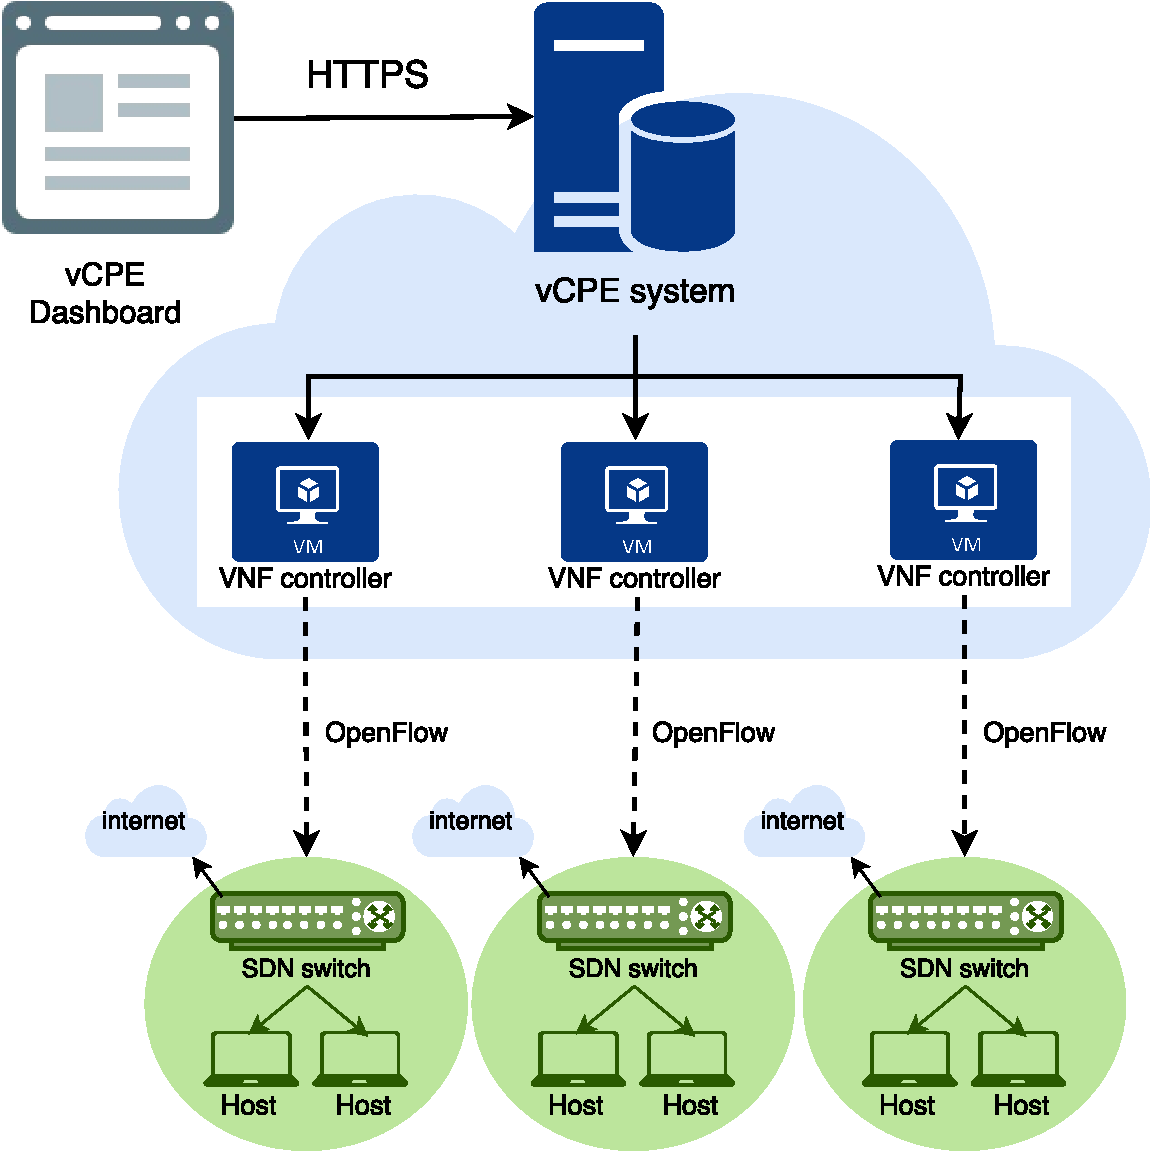
\includegraphics[width=\textwidth]{./fig/hsnl_service_deployment}
\caption{Service deployment model.}
\label{fig:hsnl_service_deployment}
\end{figure}

Fig. \ref{fig:hsnl_service_deployment} illustrates the service deployment model. Each green area is a local network domain of the customer. An SDN switch is presented at the gateway of this domain. The customer can subscribe to our vCPE service through our dashboard. After subscription, the vCPE system creates a new Docker container in which an SDN controller is run. The customer only needs to set up the gateway SDN switch to connect the SDN controller through the OpenFlow protocol; thereafter, the switch executes the service.


\subsection{Architecture of the Main System}
\subsubsection{Reference Architecture - ETSI NFV MANO Model}

\begin{figure}[!t]
\centering
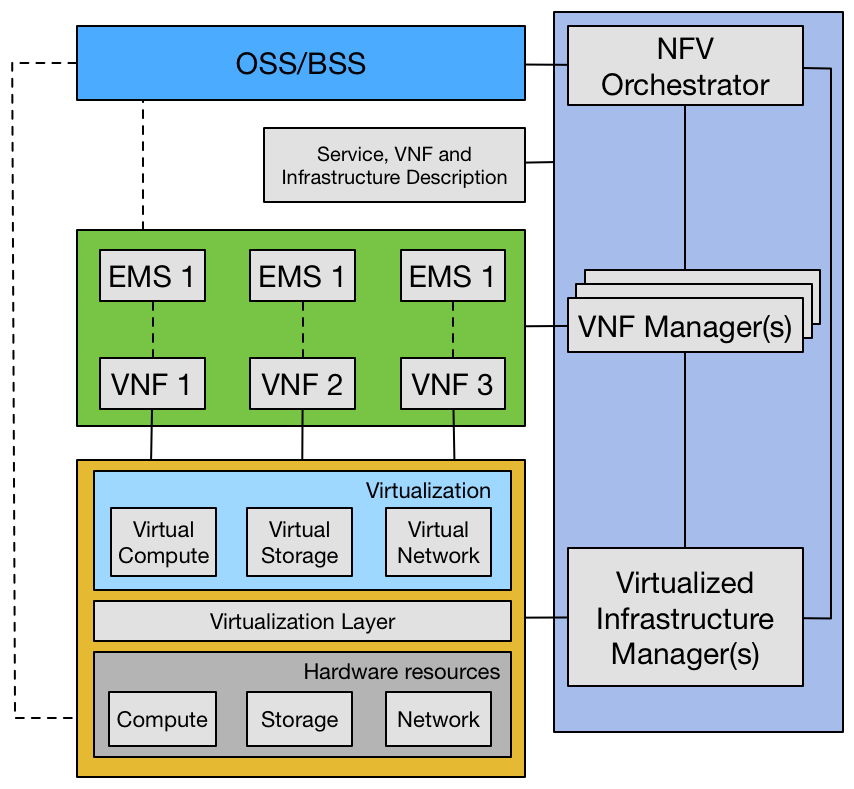
\includegraphics[width=0.8\textwidth]{./fig/etsi_nfv_architecture}
\caption{ETSI MANO Architecture.}
\label{fig:etsi_nfv_architecture}
\end{figure}

HSNL virtual CPE platform \cite{che-wei-master, che-wei-umedia} is inspired by ETSI NFV MANO model and designed under the concept of the ETSI NFV reference architectural framework \cite{etsi-nfv-archi}.

Shown in Fig. \ref{fig:etsi_nfv_architecture}, the right side of the ETSI-NFV architecture are: NFV Orchestrator (NFVO), VNF Manager (VNFM), and Virtualized Infrastructure Manager (VIM). NFVO is responsible for the orchestration and management of NFVI resources and to implement network services on the NFVI. VNFM is responsible for the lifecycle management of VNF instances (instantiation, configuration, update, scale up/down, termination, etc). VIM is responsible for controlling/managing the NFVI resources.

\subsubsection{vCPE Platform NFV Architecture}

\begin{figure}[!t]
\centering
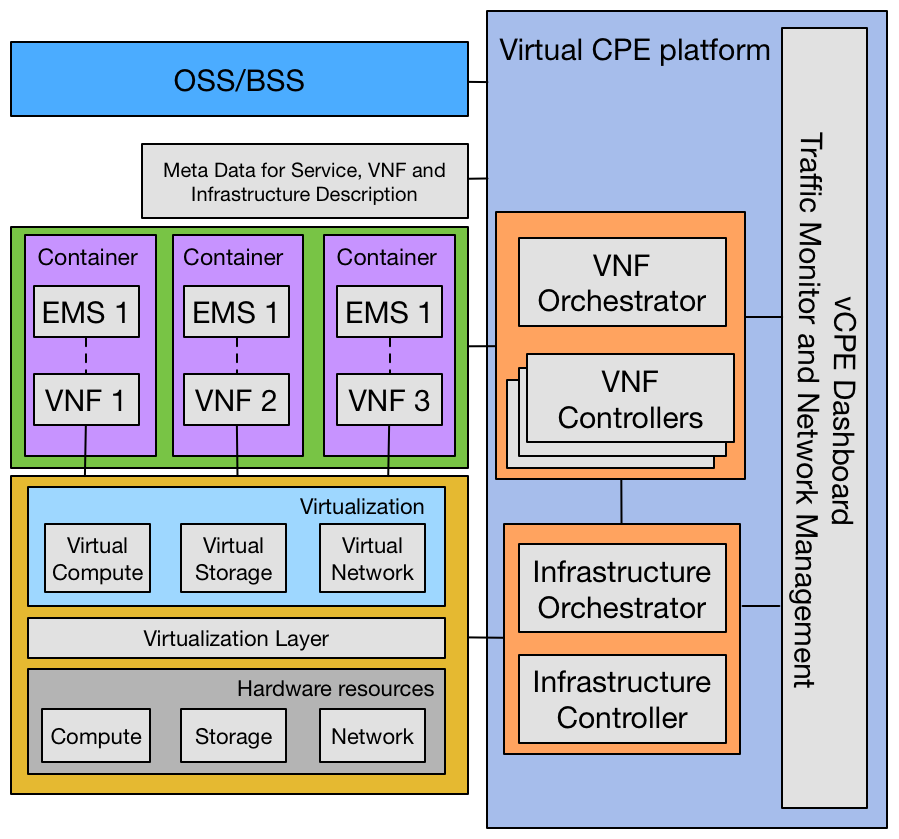
\includegraphics[width=0.8\textwidth]{./fig/hsnl_vcpe_architecture}
\caption{HSNL vCPE MANO Architecture.}
\label{fig:hsnl_vcpe_architecture}
\end{figure}

The HSNL virtual CPE architecture (Fig. \ref{fig:hsnl_vcpe_architecture}) expands the scope of ETSI NFV MANO model and we will go more detail in \ref{ssec:hsnl_system_imple}.


\subsection{System Implementation} \label{ssec:hsnl_system_imple}
Turning now to the implementation of HSNL Virtual CPE platform.  The system overview (Fig. \ref{fig:hsnl_vcpe_framework}) includes an infrastructure controller, an infrastructure orchestrator, a cloud database, VNF controllers and a VNF Orchestrator. Each component is introduced in the following subsubsection.

\begin{figure}[!t]
\centering
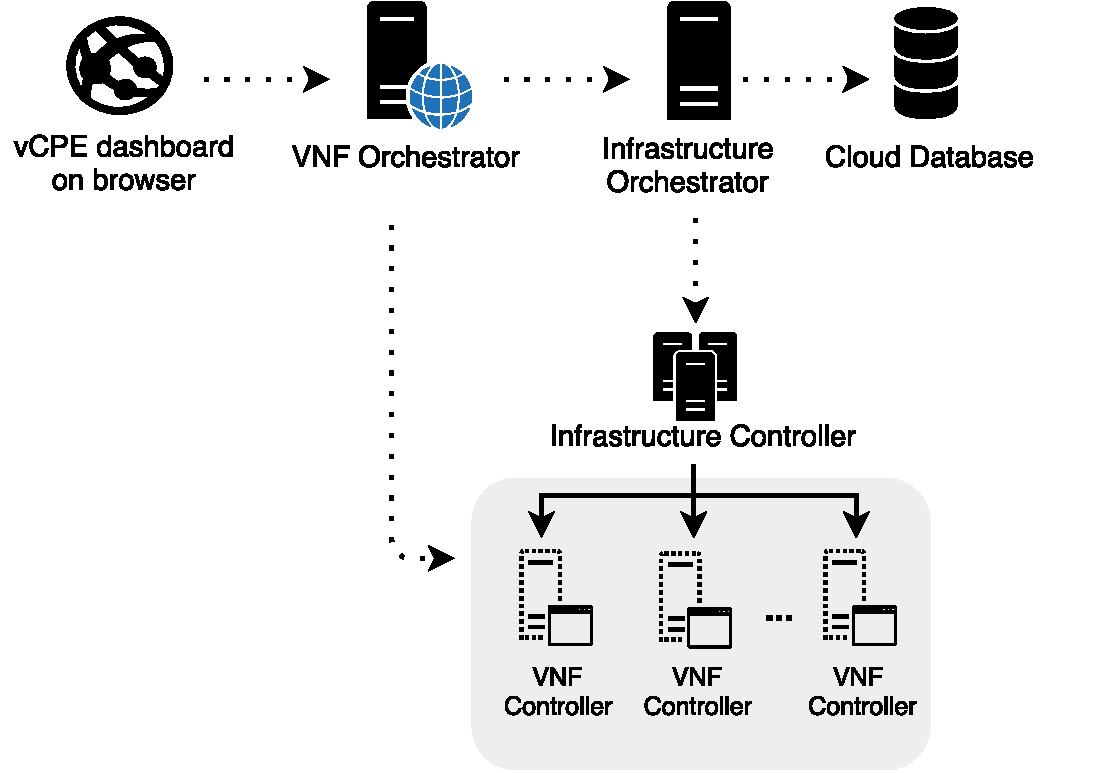
\includegraphics[width=\textwidth]{./fig/hsnl_vcpe_framework}
\caption{HSNL vCPE framework overview.}
\label{fig:hsnl_vcpe_framework}
\end{figure}

\subsubsection{Infrastructure Controller}
The infrastructure controller comprises a Docker management server that can manage the Docker resources like containers and images and a OpenStack server that can manage the VM resources. The infrastructure controller does not manage customer authentication or maintaining the state of the running service; however, it follows the request from the infrastructure orchestrator to create, delete, start, stop, and inspect containers and VMs.

\subsubsection{Infrastructure Orchestrator}
The infrastructure orchestrator plays a key role in our system. It connects and automates the workflows when our services are deployed. When a customer subscribes to our service, the infrastructure orchestrator first authenticates the customer, calls the infrastructure controller to create a container or a VM for the customer, and then updates the information in the database. The infrastructure orchestrator controls the entire life-cycle of our vCPE services.

\subsubsection{Cloud Database}
The cloud database is used for restoring the meta data of our vCPE services, which include each customer’s credentials, customer’s container/VM settings, and virtual CPE service states. The cloud database employs PostgreSQL, which is an open source, easily customizable and object-relational database system. Only the infrastructure orchestrator has permissions to access the cloud database.

\subsubsection{VNF Controllers}
VNF controllers comprises an SDN controller developed using Ryu framework \cite{ryu} and a remote launcher module. The SDN controller does not have a remote launcher module for remotely executing an SDN controller. We built a light-weight server as a launcher module to resolve this problem. The remote launcher module monitors the SDN controller process ID (PID) and kills the SDN controller PID on demand. Once the infrastructure controller  creates the container or the VM, the remote module will initially runs, waiting for requests from VNF Orchestrator. The virtual CPE functions are achieved by the synergies between the VNF controller and the SDN switch.

\subsubsection{VNF Orchestrator}
The VNF orchestrator is a web application server hosted on Amazon web server, and provides to customers an online dashboard for vCPE services management and configuration. Through the web-based UI provided by the VNF orchestrator, customers can subscribe to the desired service without typing any command through the command line interface. After receiving the subscription message, the VNF orchestrator requests the infrastructure orchestrator to create a new VNF controller, and then sends the virtual CPE configuration to the new VNF controller. Based on configuration demands under different conditions, the network administrator can select any of the listed network functions on the dashboard, such as Firewall, NAT, DHCP, quality of service (QoS) management and our proposed virtual home gateway CPE functions which is implemented by multiple flow table mechnism.
